%!TEX TS-program = xelatex
%!TEX encoding = UTF-8 Unicode

\documentclass[12pt]{article}
\usepackage{geometry}                % See geometry.pdf to learn the layout options. There are lots.
\geometry{a4paper,top=2cm}
\usepackage[parfill]{parskip}    % Activate to begin paragraphs with an empty line rather than an indent
\usepackage{graphicx}
\usepackage{amsmath}
\usepackage{amssymb}
\usepackage{mathtools}
\usepackage{physics}
\newcommand{\be}{\begin{equation}}
\newcommand{\ee}{\end{equation}}
\usepackage[thicklines]{cancel}
\usepackage[colorlinks=true,citecolor=blue,linkcolor=blue,urlcolor=blue]{hyperref}
\usepackage{booktabs}
\usepackage{csquotes}
\usepackage{qcircuit}
\usepackage{circledsteps}
\usepackage{nicefrac}
\usepackage{fontspec,xltxtra,xunicode}
\usepackage{xcolor}
\usepackage{simplewick}
\defaultfontfeatures{Mapping=tex-text}

\newcommand{\polv}{\ensuremath{\updownarrow}}
\newcommand{\polh}{\ensuremath{\leftrightarrow}}
\newcommand{\poldr}{\rotatebox[origin=c]{45}{\ensuremath{\leftrightarrow}}}
\newcommand{\poldl}{\rotatebox[origin=c]{-45}{\ensuremath{\leftrightarrow}}}
\newcommand{\bigzero}{\mbox{\normalfont\Large\bfseries 0}}
\newcommand{\vecrp}{\ensuremath{\vec{r}^{\,\prime}}}
\newcommand{\vecnr}{\ensuremath{\vec{\nabla}_{\!r}}}

\title{Advanced Quantum Mechanics\\Class 05}
%\author{The Author}
\date{August 23, 2022}                                           % Activate to display a given date or no date

\setcounter{section}{4}
\setcounter{subsection}{2}
\setcounter{equation}{22}

\begin{document}
\maketitle
\subsection{Spin-1/2 in a periodic magnetic field}

Atomic nucleus with nonzero spin.
Limit discussion to spin-1/2 nuclei ($H$,$^{13}C$,$^{19}F$,\ldots),
they have magnetic moment $\vec{\mu}$ $\to$ operator in QM: 
\be
\hat{\vec{\mu}}=\gamma \hat{\vec{s}}=\frac{1}{2} \gamma \hbar \vec{\sigma}
\ee

\be
\gamma=\bar{\gamma} \frac{q_{p}}{2 m_{p}}\left\{\begin{array}{l}\bar{\gamma} \text { proton: } 5.59 \\ \bar{\gamma} \, { }^{13} C: 1.40\end{array}\right.
\ee

Nuclear spin in a $\vec{B}_0=B_{0} \hat{z}$:
\be
\begin{aligned} 
H_{0} &=-\vec{\mu} \cdot \vec{B}=-\frac{1}{2} \gamma \hbar B_{0} \sigma_{z} 
\\
&\to \gamma B_0 \equiv \omega_0 \text{ no minus sign, } q_p > 0
\\ 
&=-\frac{1}{2} \hbar \omega_{0} \sigma_{z} 
\end{aligned}
\ee
therefore
\be
H_{0}=-\frac{1}{2} \hbar
\begin{pmatrix}
\omega_{0} & 0 \\ 0 & -\omega_{0}
\end{pmatrix}
\ee
and we have the basis eigenstates
\be
\left.
\begin{array}{l}
|+\rangle \rightarrow\left(\begin{array}{l}1 \\ 0\end{array}\right) \therefore-\hbar \omega_{0} / 2 \\ 
|-\rangle \rightarrow\left(\begin{array}{l}0 \\ 1\end{array}\right) \therefore+\hbar \omega_{0} / 2
\end{array}\right\}
\to \text{ Zeeman levels}
\ee

Add a time-dependent field $\vec{B}_{1}(t)$ parallel
to the $xOy$ plane, rotating clockwise direction,
%%% 2
with frequency $\omega$:
\be
\vec{B}_{1}(t)=B_{1}(\cos \omega t \hat{x}-\sin \omega t \hat{y})
\ee
(the minus sign indicates clockwise motion). Therefore
\be
\begin{aligned} \hat{H}_{1}(t) 
&=-\vec{\mu} \cdot \vec{B}_{1}  (t)=-\gamma \vec{B}_{1}(t) \cdot \vec{S} \\ 
&=-\frac{1}{2} \underbrace{\gamma \hbar B_{1}}_{\gamma B_{1} \equiv \omega_{1}} \left(\cos \omega t \, \sigma_{x}-\sin \omega t \, \sigma_{y}\right) \\ 
&=-\frac{1}{2} \hbar \omega_{1}
\begin{pmatrix} 
0 & \cos \omega t+i \sin \omega t \\ 
\cos \omega t-i \sin \omega t & 0
\end{pmatrix}
\end{aligned}
\ee
leading to the full Hamiltonian
\be
\hat{H}(t)=\hat{H}_{0}+\hat{H}_{1}(t)=
-\frac{1}{2} \hbar
\begin{pmatrix}
\omega_{0} & \omega_{1} e^{i \omega t} \\ 
\omega_{1} e^{-i \omega t} & -\omega_{0}
\end{pmatrix}
\ee
The Schrödinger equation (matrix form)
\be
|\psi(t)\rangle=c_{+}(t)|+\rangle+c_{-}(t)|-\rangle
\label{eq:g31}
\ee
\[
\begin{aligned} 
i \hbar \frac{d}{d t}|\psi(t)\rangle 
&=i \hbar\left(\dot{c}_{+}(t)|+\rangle+c_{-}(t)|-\rangle\right) \\ 
&=-\frac{1}{2} \hbar
\begin{pmatrix}
\omega_{0} & \omega_{1} e^{i \omega t} \\ 
\omega_{1} e^{-i \omega t} & -\omega_{0}
\end{pmatrix} 
\begin{pmatrix}
c_{+}(t) \\ 
c_{-}(t)
\end{pmatrix} 
\end{aligned}
\]
and therefore
\be
\begin{aligned}
i \dot{c}_{+}(t)&=-\frac{1}{2}\left[\omega_{0} c_{+}(t)+\omega_{1} e^{i \omega t} c_{-}(t)\right]\\
i \dot{c}_{-}(t)&=-\frac{1}{2}\left[\omega_{1} e^{-i \omega t} c_{+}(t)-\omega_{0} c_{-}(t)\right]
\end{aligned}
\ee
%%% 3
leading finally to
\be
\boxed{
i \dot{c}_{\pm}(t)=\mp \frac{1}{2} \omega_{0} c_{\pm}(t)-\frac{1}{2} \omega_{1} e^{\pm i \omega t} c_{\mp}(t)
}
\label{eq:g33}
\ee
Solution: propose 
\be
c \pm(t)=\gamma_{\pm}(t) e^{\pm i \omega_{0} t / 2}
\ee
and replace  this in Eq.~\eqref{eq:g33}:
\[
\begin{gathered}
i \dot{\gamma_{\pm}}(t) e^{\pm i\omega_0 t/2} 
\mp \cancel{\frac{\omega_0}{2} \gamma_{\pm}(t) e^{\pm i\omega_0 t/2}}
=
\mp \cancel{\frac{1}{2} \omega_0 \gamma_{\pm}(t) e^{\pm i\omega_0 t/2}}\\
-\frac{1}{2} \omega_{1}e^{\pm i\omega t} \gamma_{\mp} (t) e^{\mp i\omega_0 t/2} 
\end{gathered}
\]
hence
\be
i \dot{\gamma_{\pm}}(t) = -\frac{1}{2} \omega_1 e^{\pm i\left(\omega-\omega_{0}\right) t}
\gamma_{\mp}(t)
\label{eq:g35}
\ee
where we can identify the \emph{detuning} frequency:
\be
\delta = \omega - \omega_0
\ee

\subsubsection{On-resonance case}

Let us solve this \emph{first} for $\delta = 0$, the \emph{on-resonance} case:
\[
i \gamma_{\pm}=-\frac{1}{2} \omega_{1} \dot{\gamma}_{\mp}=-\frac{1}{2} \omega_{1}\left(+\frac{1}{2} i \omega_{1} \gamma_{\pm}\right)
\]
where we now use Eq.~\eqref{eq:g35}, hence
\be
\boxed{
i \ddot{\gamma}_{\pm}+ \frac{1}{4}\omega_{1}^{2} \gamma_{\pm}=0
}
\ee

Solution:
\be
\begin{aligned}
\gamma_{+}(t)&=a \cos \omega_{1} t / 2+b \sin \omega_{1} t / 2\\
\gamma_{-}(t)&=-\frac{2 i}{\omega_{1}} \dot{\gamma}_{+}=i a \sin \omega_{1} t / 2-i b \cos \omega_{1} t / 2
\end{aligned}
\label{eq:g38}
\ee
and therefore, for $\ket{\psi(t)}$, from Eq.~\eqref{eq:g31}
\be
|\psi(t)\rangle=\gamma_{+}(t) e^{i \omega_{0} t / 2}|+\rangle+\gamma_{-}(t) e^{-i \omega_{0} t / 2}|-\rangle
\ee

%%% 4 OK

Suppose $t=0$, system in lowest energy state:
\[
E_{0}=-\hbar \omega_{0} / 2 \Rightarrow|\psi(0)\rangle=|+\rangle
\]
\[
|\psi(0)\rangle=
\underbrace{\gamma_+(0)}_{1} \ket{+} + 
\underbrace{\gamma_-(0)}_{0} \ket{-}
\]
hence
\be
1=a,\,0=-ib \quad \therefore \quad \boxed{a=1,\,b=0}
\ee
and finally
\be
|\psi(t)\rangle=
\cos \omega_{1} t / 2 e^{ i \omega_{0} t / 2}|+\rangle+i 
\sin \omega_{1} t / 2 e^{-i \omega_{0} t / 2}|-\rangle
\ee
Probabilities $p_\pm(t)$ of finding the spin in
states $\ket{\pm}$ are:
\be
\begin{aligned}
p_{+}(t)&=|\langle+|\psi(t)\rangle|^{2}&=\cos ^{2} \omega_{1} t / 2 \\ 
p_{-}(t)&=|\langle-|\psi(t)\rangle|^{2}&=\sin ^{2} \omega_{1} t / 2
\end{aligned}
\label{eq:g42}
\ee

%%% 5 OK

Recall: $\delta = 0 \Rightarrow \omega = \omega_0,\quad \omega_1 = \gamma B_1$.
From Eq.~\eqref{eq:g42}, we see oscillations between energy
levels $\pm E_0 = \pm \hbar\omega_0/2$ $\to$ Rabi oscillations.
Spin initially ($t=0$) in $\ket{+}$ will be
found in $\ket{-}$ when $\sin ^{2} \omega_{1} t / 2=1$.
\[
\frac{\omega_{1} t}{2}=(2 n+1) \pi / 2=(n+1 / 2) \pi, n=0,1, \ldots
\]
$\to$ $\vec{B_1}(t)$ satisfying this: $\pi$-pulse

When 
\be
\omega_{1} t / 2=(n+1 / 2) \pi / 2,
\ee
a $\pi/2$ pulse, we have
\[
\cos ^{2}(n+1 / 2) \pi / 2=\frac{1}{2} \quad 
\sin ^{2}(n+1 / 2) \pi / 2=\frac{1}{2}
\]
and therefore
\be
\frac{1}{\sqrt{2}}
[\ket{+} \pm \ket{-}]
\ee

\subsubsection{Neat geometrical interpretation}

We have
\[
C_{\pm}(t)=\gamma_{\pm}(t) e^{\pm i \omega_{0} t / 2}.
\]
If $\vec{B_1} = 0$, $\gamma_\pm$ are time-independent 
$\to$ the spin performs Larmor precession
about $\vec{B_0}$, clockwise, with frequency $\omega_0$.
%%% 6 OK
Instead using the lab frame to measure $x$ and $y$
components of spins $\to$ use the frame rotating
around $O_z$ with frequency $\omega_0$; this amounts
to change $\ket{\psi(t)} \to \ket{\psi^\prime(t)}$ [see chapter on rotations]:
\[
\begin{aligned}
\left|\psi^{\prime}(t)\right\rangle
&=\overbrace{e^{-i \omega_{0} t / 2 \sigma_{z}}}%
^{\text{rotation operator}}
|\psi(t)\rangle\\
&=\underbrace{c_{+}(t) e^{-i \omega_{0} t / 2}}%
_{\gamma_+(t)}|+\rangle
 +\underbrace{c_{-}(t) e^{i \omega_{0} t / 2}}%
_{\gamma_-(t)}|-\rangle
\end{aligned}
\]
$\gamma_\pm(t)$: are just the components of 
the state vector in the rotation
frame of reference.
Analogously for Eq.~\eqref{eq:g38}:
\[
\begin{pmatrix}
\gamma_+(t)\\
\gamma_-(t)
\end{pmatrix}
U[R_x(-\theta)]
\begin{pmatrix}
\gamma_+(0)\\
\gamma_-(0)
\end{pmatrix}
\]
where $\begin{pmatrix}
\gamma_+(0)\\
\gamma_-(0)
\end{pmatrix} = 
\begin{pmatrix}
a\\
-ib
\end{pmatrix}
$ and $\theta = \omega_1 t$.
The operator $U[R_x(-\theta)]$ is
\[
U[R_x(-\theta)] = e^{-i(-\theta)/2 \sigma_x} = 
\begin{pmatrix}
\cos \theta/2 & i \sin \theta/2\\
i \sin \theta/2 & \cos \theta/2
\end{pmatrix}
\]

\subsubsection{Off-resonance case}

Suppose now $\delta \neq 0$, the \emph{off-resonance} case.
For a solution: differentiate Eq.~\eqref{eq:g35} and use it again:
\[
i \ddot{\gamma}_{\pm}=\mp \frac{1}{2} i \omega_{1} \delta e^{\pm i \delta t} \gamma_{\mp}-\frac{1}{2} \omega_{1} e^{\pm i \delta t} \dot{\gamma}_{\mp}
\]
%%% 7
and
\[
\begin{gathered}
i \ddot{\gamma}_\pm = \mp \frac{1}{2} i \omega_1 \delta 
\cancel{e^{\pm i \delta t}}
\left[
-\frac{2i}{\omega_1} \cancel{e^{\mp i \delta t}}
\dot{\gamma}_\pm
\right]\\
-\frac{1}{2} \omega_1 \cancel{e^{\pm i \delta t}}
\left[
+\frac{i \omega_1}{2} \cancel{e^{\mp i \delta t}}
\gamma_\pm
\right]
\end{gathered}
\]
and finally, focussing on $\gamma_+$ for the moment,
\be
\boxed{
\ddot{\gamma}_{+}-i \delta \dot{\gamma}_{+}+ \frac{1}{4} \omega_{1}^{2} \gamma_{+}
}
\ee
Propose solution in the form
\be
\gamma_{+}=e^{i \Omega_{\pm} t}
\ee
\[
-\Omega_{\pm}^{2}+\delta \Omega_{\pm} +1/4 \omega_{1}^{2}=0
\]
\[
\Omega_{\pm}^{2}-\delta \Omega_\pm -1/4 \omega_{1}^{2}=0 \Rightarrow \Omega_{\pm}= 1/2
\left(\delta \pm \sqrt{\delta^{2}+\omega_{1}^{2}}\right)
\]
\be
\Omega \equiv \sqrt{\delta^{2}+\omega_{1}^{2}}=\sqrt{\left(\omega-\omega_{0}\right)^{2}+\omega_{1}^{2}}
\ee
finally leading to
\be
\gamma_{+}(t)=\lambda e^{i \Omega_{+} t}+\mu e^{+i \Omega_{-} t}
\ee
and $\gamma_{-}(t)$ from Eq.~\eqref{eq:g35}:
\be
\gamma_{-}(t)=
-\frac{2 i}{\omega_{1}} e^{-i \delta t} \dot{\gamma}_{+}=
-\frac{2 i}{\omega_{1}} 
\left( 
i \Omega_{+} \lambda e^{i \Omega_{+} t} +
i \Omega_{-} \lambda e^{i \Omega_{-} t}
\right)
e^{-i \delta t}
\ee
%%% 8
\be
\gamma_{-}(t)=\frac{2 \Omega_{+}}{\omega_{1}} \lambda e^{i\left(\Omega_{+}-\delta\right) t}+\frac{2 \Omega_{-}}{\omega_{1}} e^{i\left(\Omega_{-}-\delta\right) t}
\ee

Suppose $t=0$: $\ket{\psi(0}) = \ket{+}$
\[
\ket{+}=
\underbrace{\gamma_+(0)}_{1} \ket{+}+ 
\underbrace{\gamma_-(0)}_{0} \ket{-} 
\]
Now have to solve for $\lambda$ and $\mu$.
\[
\begin{gathered}
\lambda+\mu=1 \quad \therefore \quad \frac{2 \Omega_{+}}{\omega_{1}} \lambda+\frac{2 \Omega_-}{\omega_{1}} \mu=0\\
\Omega_+\lambda+\Omega_-\mu=0
\end{gathered}
\]
\[
\lambda+\frac{\Omega_{-}}{\Omega_{+}} \mu=0 
\therefore\left(1-\frac{\Omega_{-}}{\Omega_{+}}\right) \mu=1
\]
\be
\underbrace{(\Omega_{+} + \Omega_{-})}%
_{\Omega}
\mu = \Omega_{+}
\therefore
\mu = \frac{\Omega_{+}}{\Omega}
\ee
and
\be
\lambda=-\frac{\Omega_{-}}{\Omega_{+}} \mu=-\frac{\Omega_{-}}{\Omega_{+}} \frac{\Omega_{+}}{\Omega}=
\frac{\Omega_{-}}{\Omega}
\ee
Finally
\be
\lambda=-\frac{\Omega_{-}}{\Omega}=-\frac{1}{2 \Omega}(\delta-\Omega)=\frac{1}{2}-\frac{\delta}{2 \Omega}
\ee
\be
\lambda=-\frac{\Omega_{+}}{\Omega}= \frac{1}{2 \Omega}(\delta+\Omega)=\frac{1}{2}+\frac{\delta}{2 \Omega}
\ee
and therefore
\[
\begin{aligned}
\gamma_{+}(t)
&=\left(\frac{1}{2}-\frac{\delta}{2 \Omega}\right) e^{i(\delta+\Omega) t / 2}+\left(\frac{1}{2}+\frac{\delta}{2 \Omega}\right) e^{i(\delta-\Omega) t / 2}\\
&=\frac{e^{i \delta t / 2}}{\Omega}\left[\frac{\Omega}{2}\left(e^{i \Omega t / 2}+e^{-i \Omega t / 2}\right)
-
\frac{\delta}{2}\left(e^{i \Omega t / 2}-e^{-i \Omega t / 2}\right)\right]
\end{aligned}
\]
\be
\boxed{
\gamma_{+}(t)=\frac{e^{i \delta t / 2}}{\Omega}[\Omega \cos (\Omega t / 2)-i \delta \sin (\Omega t / 2)]
}
\ee
\emph{Exercise:} show that
\be
\boxed{
\gamma_{-}(t)=\frac{i \omega_{1}}{\Omega} e^{-i \delta t / 2} \sin (\Omega t / 2)
}
\ee

Probabilities:
\[
\begin{aligned}
p_+(t) 
&= |\bra{+}\ket{\psi(t)}|^2 = |\gamma_+(t)|^2\\
&=\frac{1}{\Omega^{2}}\left[\Omega^{2} \cos (\Omega t / 2)+\delta^{2} \sin ^{2}(\Omega t / 2)\right]\\
&=\frac{1}{\Omega^{2}}\left[\left(\delta^{2}+\omega_{1}^{2}\right) \cos ^{2}(\Omega t / 2)+\delta^{2} \sin ^{2}(\Omega t / 2)\right]\\
&=\frac{1}{\Omega^{2}}\left[\delta^{2}+\omega_{1}^{2} \cos ^{2}(\Omega t / 2)\right]
\end{aligned}
\]
Therefore:
\be
p_{+}(t)=\frac{\omega_{1}^{2}}{\omega_{1}^{2}+\delta^{2}}\left[\cos ^{2}(\Omega t / 2)+\frac{\delta^{2}}{\omega_{1}^{2}}\right]
\ee
and
\be
p_{-}(t)=\frac{\omega_{1}^{2}}{\omega_{1}^{2}+\delta^{2}} \sin ^{2}(\Omega t / 2)
\ee
The maximum probability for a transition
from $\ket{+}$ to $\ket{-}$ occurs for
\be
\left(p_{-}\right)_{\max} \Rightarrow 
\frac{\Omega t}{2} = \frac{\pi}{2}
\ee
We can see the effects of going off-resonance:
\begin{center}
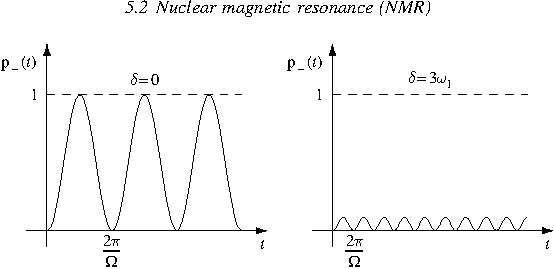
\includegraphics[width=0.8\textwidth]{Figures/RabiOscillations.pdf}
\end{center}

\emph{Homework:} read the text on the nuclear magnetic resonance (NMR).

\clearpage

%%% 11

\subsection{Two-level systems with electric dipole moment}

Under the influence of external electric field.
Example of a physical system: ammonia molecule.
\begin{center}
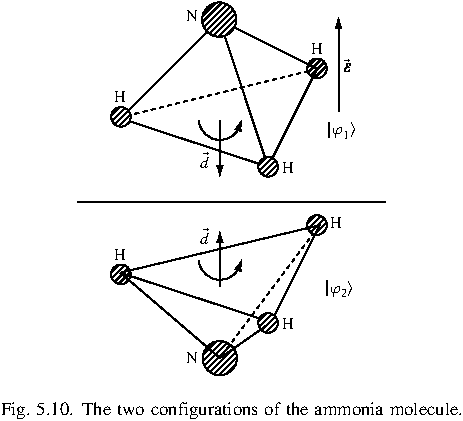
\includegraphics[width=0.5\textwidth]{Figures/ammoniaMolecule.pdf}
\end{center}
It forms a molecule with a \emph{dipole moment} $\vec{d}$,
perpendicular to the plane formed by the hydrogen atoms. The nitrogen atom can oscillate through that plane.

In the absence of an external electric field:
\be
H=H_{0}+H^{\prime}=
\begin{pmatrix}
E_{0} & 0 \\ 0 & E_{0}
\end{pmatrix}
+
\begin{pmatrix}
0 &-A \\ -A & 0
\end{pmatrix}
=
\begin{pmatrix}
E_{0} & -A \\ -A & E_{0}
\end{pmatrix}
\ee
$A$: what causes the N atom to cross the plane.

%% 12
\be
\left\{\left|\varphi_{1}\right\rangle,\left|\varphi_{2}\right\rangle\right\} 
\text { eigenstates of } H_{0},
\left|\varphi_{1}\right\rangle=\left(\begin{array}{l}1 \\ 0\end{array}\right), 
\left|\varphi_{2}\right\rangle=\left(\begin{array}{l}0 \\ 1\end{array}\right)
\ee
%
\[
\left\{\left|\chi_{+}\right\rangle,\left|\chi_{-}\right\rangle\right\}  
\text { eigenstates of } H
\]
leading to
\[
\begin{aligned}
|\chi_{+}\rangle&=\frac{1}{\sqrt{2}}\left(\left|\varphi_{1}\right\rangle+\left|\varphi_{2}\right\rangle\right)=\frac{1}{\sqrt{2}}\begin{pmatrix}1 \\ 1\end{pmatrix}, 
&\quad E=E_{0}-A \\
|\chi_{-}\rangle&=\frac{1}{\sqrt{2}}\left(\left| \varphi_{1}\right\rangle-\left|\varphi_{2}\right\rangle\right)=\frac{1}{\sqrt{2}}\begin{pmatrix}1 \\ -1\end{pmatrix},
&\quad E=E_{0}+A
\end{aligned}
\]

%%% Pra ficar igual às notas do Gastão
\setcounter{equation}{62}

\emph{Apply an electric field:} $\vec{\epsilon} = |\vec{\epsilon}|\hat{z}$.
\[
\text { Empirical fact }\left\{\begin{array}{ll}\left|\varphi_{1}\right\rangle & \text { has } \vec{d} \sim-\hat{z} \\ \left|\varphi_{2}\right\rangle & \text { has } \vec{d} \sim+\hat{z}\end{array}\right.
\]
Potential energy:
\be
E = -\vec{d}\cdot\vec{\epsilon}
\ee
so the energy is minimised when $\vec{d} \parallel \vec{\epsilon}$.
\be
\begin{array}{l}
\left|\varphi_{1}\right\rangle: \vec{d} \sim-\vec{z} \Rightarrow E_{1}=E_{0}+d \varepsilon \\ 
\left|\varphi_{2}\right\rangle: \vec{d} \sim+\vec{z} \Rightarrow E_{2}=E_{0}-d \varepsilon
\end{array}
\ee
\be
H=\left(\begin{array}{cc}E_{0}+d \varepsilon & -A \\ -A & E_{0}-d \varepsilon\end{array}\right)
\ee

\subsubsection{Static $\vec{\varepsilon}$}

Eigenvalues $E$ $\to$ $\det H = 0$.
\[
\begin{array}{r}\left(E_{0}+d \varepsilon-E\right)\left(E_{0}-d \varepsilon-E\right)-A^{2}=0 \\ {\left[\left(E_{0}-E\right)+d \varepsilon\right]\left[\left(E_{0}-E\right)-d \varepsilon\right]-A^{2}=0}\end{array}
\]
Recall the sign convention:
\[
\begin{array}{l}
\left|\chi_{+}\right\rangle \rightarrow E_{0}-A \\ 
\left|\chi_{-}\right\rangle \rightarrow E_{0}+A
\end{array}
\]
hence
\be
\left(E_{0}-E\right)^{2}=A^{2}+(d \varepsilon)^{2} \therefore E_{\pm}=E_{0} \mp \sqrt{A^{2}+(d \varepsilon)^{2}}
\ee
\be
E_{\pm}=
\left\{
\begin{aligned}
&E_{0} \mp d \varepsilon, &\frac{d \varepsilon}{A}\gg1 \\
&\left(E_{0} \mp A\right) \mp 1 / 2 \frac{(d \varepsilon)^{2}}{A^{2}}, &\frac{d \varepsilon}{A}\ll1
\end{aligned}
\right.
\ee

\begin{center}
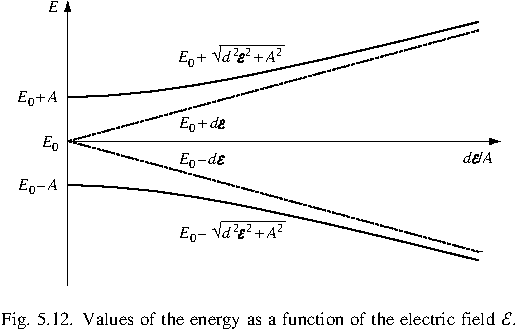
\includegraphics[width=0.8\textwidth]{Figures/ammoniaLevels.pdf}
\end{center}

$E+\rightarrow\left|\chi_{+}\right\rangle \quad E_{-} \rightarrow\left|\chi_{-}\right\rangle$ up to terms
of order $d\epsilon/2A$ $\to$ $\ket{\chi_+^{\prime}} =
\begin{pmatrix}
1-d\epsilon/2A\\1+d\epsilon/2A
\end{pmatrix}
$, as can be seen in Exercise 5.54.

%%% Pra ficar igual às notas do Gastão
\setcounter{equation}{66}
The spectrum can be measured using the analogue
to a Stern-Gerlach experiment $B \to E$
\be
\vec{F}_\pm = -\vec{\nabla}E_\pm=
\frac{d^{2}}{A} \vec{\varepsilon} \cdot \vec{\nabla} \varepsilon
\ee

%%% 14

\subsubsection{Time dependent electric field}

\be
\varepsilon(t)=\varepsilon_{0} \cos \omega t=\frac{1}{2} \varepsilon_{0}\left(e^{i \omega t}+e^{-i \omega t}\right),
\, \varepsilon_{0}\text{ real}
\ee
Write Hamiltonian in the $\{\ket{\chi_+},\ket{\chi_-}\}$ basis:

\be
H(t)=\begin{pmatrix}
E_{0}-A & d \varepsilon(t) \\ 
d \varepsilon(t) & E_{0}+A
\end{pmatrix}
\ee

\be
\ket{\psi(t)} = c_+(t)\ket{\chi_+} + c_-(t)\ket{\chi_-}
\ee
\[
i\hbar \frac{d}{d t} \ket{\psi(t)} = 
\begin{pmatrix}
E_{0}-A & d \varepsilon(t) \\ 
d \varepsilon(t) & E_{0}+A
\end{pmatrix}
\left(
c_+(t)\ket{\chi_+} + c_-(t)\ket{\chi_-}
\right)
\]
hence
\be
\begin{aligned}
i \hbar \dot{c}_{+}(t)&=\left(E_{0}-A\right) c_{+}(t)+d \varepsilon(t) c_{-}(t) \\
i \hbar \dot{c}_{-}(t)&=d \varepsilon(t) c_{+}(t)+\left(E_{0}+A\right) c_{-}(t)
\end{aligned}
\ee
and when $\varepsilon = 0$
\be
\begin{aligned} 
c_{+}(t) \sim e^{-i / \hbar\left(E_{0}-A\right) t} &=e^{-i \omega_{+} t} \\ 
c_{-}(t) \sim e^{-i / \hbar\left(E_{0}+A\right) t} &=e^{-i \omega_{-} t} 
\end{aligned}
\ee
with
\be
\omega_{\pm}=\left(E_{0} \mp A\right) / \hbar
\ee

%%% 15

For $\varepsilon = 0$, propose
\be
c_{\pm}(t)=\gamma_{\pm}(t) e^{-i \omega \pm t}
\ee
Substituting these in, similar to NMR:
\be
\begin{aligned}
i \dot{\gamma}_{\pm}
&=\frac{1}{\hbar} \dot{\varepsilon}(t) e^{\mp i \omega_{0} t} \gamma_{\mp},\,
\boxed{
\omega_{0}=2 A / \hbar
}\\
&=\frac{1}{2} 
\underbrace{\frac{d \varepsilon_{0}}{\hbar}}%
_{\omega_1}
\left[
e^{ i\left(\omega\mp \omega_{0}\right) t}+
e^{-i\left(\omega\pm \omega_{0}\right) t}
\right] \gamma_{\mp}(t) 
\end{aligned}
\ee
where 
\be
\omega_1 \simeq \text{ ``Rabi'', causes transitions }
\left\{
\begin{gathered}
E_0-A\\
E_0+A
\end{gathered}
\right. 
\ee
And this cannot be solved analytically.

Two approximations:
\begin{enumerate}
\item\emph{weak field:}
\be
d\varepsilon_{0} \ll A \rightarrow \frac{d \varepsilon_{0}}{\hbar} \ll \frac{A}{\hbar} \sim \omega_{0}
\ee
Rabi frequency: $\omega_{1}=d \varepsilon_{0} / \hbar \ll \omega_{0}$
\item\emph{close to resonance:}
\be
\omega \simeq \omega_0 \rightarrow \delta = (\omega-\omega_0)\text{ small}
\ee
\end{enumerate}

\begin{enumerate}
\item Weak field $\to$ $\gamma_\pm(t)$ slowly-varying,
would not vary at all if $\varepsilon = 0$ 
\be
|\dot{\gamma}_{\pm}|
\sim \omega_{1} |\gamma_{\mp}|
\ll
\omega_{0}|\gamma_{\mp}|
\ee
%%% Pra ficar igual às notas do Gastão
\setcounter{equation}{78}
\item $\omega \simeq \omega_0$: 
\be
e^{\pm i\left(\omega_{0}+\omega\right) t} \approx e^{\pm 2 i \omega_{0} t}
\ee
therefore
%%% 16
\be
\begin{gathered}
i \dot{\gamma}_{+} \approx \frac{1}{2} \omega_{1}\left(e^{i \delta t}+e^{-2 i \omega_{0} t}\right) 
\approx \frac{1}{2} \omega_{1} e^{i \delta t} \gamma_{-}\\
i \dot{\gamma}_{-} \approx \frac{1}{2} \omega_{1}\left(e^{2 i \omega_{0} t}+e^{-i \delta t}\right)
\approx \frac{1}{2} \omega_{1} e^{-i \delta t} \gamma_{+}
\end{gathered}
\ee
and finally 
\be
i \dot{\gamma}_{\pm}=\frac{\omega_{1}}{2} e^{i \delta t} \gamma_{\mp}
\ee
that is identical to NMR (up to an irrelevant minus sign).
\end{enumerate}

Suppose for now:
\[
\omega=\omega_{0} \rightarrow \delta=0, \quad 
t=0 \quad|\psi(0)\rangle=|\chi_{-}\rangle
\]
with energy $E_- = E_0+A$.
Notice that this the opposite situation from Eq.~\eqref{eq:g42}. Then:
\be
\begin{aligned}
p_{-}(t)&=\left|\left\langle \chi_{-} \mid \psi(t)\right\rangle\right|^{2}=\cos ^{2}(\omega_1 t / 2) \\ 
p_{+}(t)&=\left|\left\langle \chi_{+} \mid \psi(t)\right\rangle\right|^{2}=\sin ^{2}(\omega_1 t / 2)\
\end{aligned}
\ee
The molecule goes from $\ket{\chi_-}$ to $\ket{\chi_+}$
with frequency $\omega_1/2 = d \varepsilon_{0} / 2 \hbar$ 
$\to$ stimulated emission/absorption.
%%% 17
Prepare molecules in $\ket{\chi_-}$ (excited state)
-- the fact that the majority of the molecules are in the excited state is the \emph{population inversion};
pass them through a cavity where there is an $\varepsilon(t)$
with frequency $\omega \approx \omega_{0}=2 A / \hbar$. The molecule
crosses the cavity in a time interval $t$.
If this time is adjusted such that $\frac{\omega_{1} t}{2}=\pi / 2$
\be
\frac{\omega_{1} t}{2}=\frac{d \varepsilon_{0}}{2 \hbar} t=\frac{\pi}{2}
\ee
all molecules that have passed through the cavity will be $\ket{\chi_+}$:
$\ket{\chi_-}\rightarrow\ket{\chi_+}, E_{-} > E_{+}$, emission of photons -- \emph{stimulated emission}.
The reverse process $\to$ \emph{stimulated absorption}.
This is a prototype of a \emph{maser}:
microwave amplification by stimulated emission of radiation.
For a \emph{laser}, microwave $\to$ light.

\end{document} 